\section{Patterns}

\begin{frame}{Wire-based microstructures}
% Large examples of wire-based microstructure
\begin{figure}
\includegraphics[width=0.8\textwidth]{Images/diamond_cube.png}
\end{figure}
\end{frame}

\begin{frame}{Wire-based microstructures}
% motivation of using wire-based structures.
\begin{figure}
\centering
\hspace{\fill}
\includegraphics[width=0.4\textwidth]{Images/molecular_structures.png}
\hspace{\fill}
\pause \includegraphics[width=0.4\textwidth]{Images/javits_center.png}
\hspace{\fill}

\vspace{3mm}
\pause \includegraphics[width=0.9\textwidth]{Images/sponge_structure.pdf}
\end{figure}
\end{frame}

\begin{frame}{Single cell patterns}
% Show a few single cell patterns
% brick5, diamond, star, truncated octahedron
\begin{figure}
\hspace{\fill}
\includegraphics[width=0.4\textwidth]{Images/brick5_cell.png}
\hspace{\fill}
\includegraphics[width=0.4\textwidth]{Images/star_cell.png}
\hspace{\fill}

\vspace{3mm}
\hspace{\fill}
\includegraphics[width=0.4\textwidth]{Images/truncated_octahedron_cell.png}
\hspace{\fill}
\includegraphics[width=0.4\textwidth]{Images/diamond_cell.png}
\hspace{\fill}
\end{figure}
\end{frame}

\begin{frame}{Single cell patterns}
% Show a few single cell patterns
% brick5, diamond, star, truncated octahedron
\begin{figure}
\hspace{\fill}
\includegraphics[width=0.4\textwidth]{Images/brick5_cell_source.png}
\hspace{\fill}
\includegraphics[width=0.4\textwidth]{Images/star_cell_source.png}
\hspace{\fill}

\vspace{3mm}
\hspace{\fill}
\includegraphics[width=0.4\textwidth]{Images/truncated_octahedron_cell_source.png}
\hspace{\fill}
\includegraphics[width=0.4\textwidth]{Images/diamond_cell_source.png}
\hspace{\fill}
\end{figure}
\end{frame}

\begin{frame}{Inflation}
% Illustrate the steps
\begin{figure}
\centering
\hspace{\fill}

\includegraphics[width=0.3\textwidth]{Images/inflation_0.pdf}
\hspace{\fill}
\pause 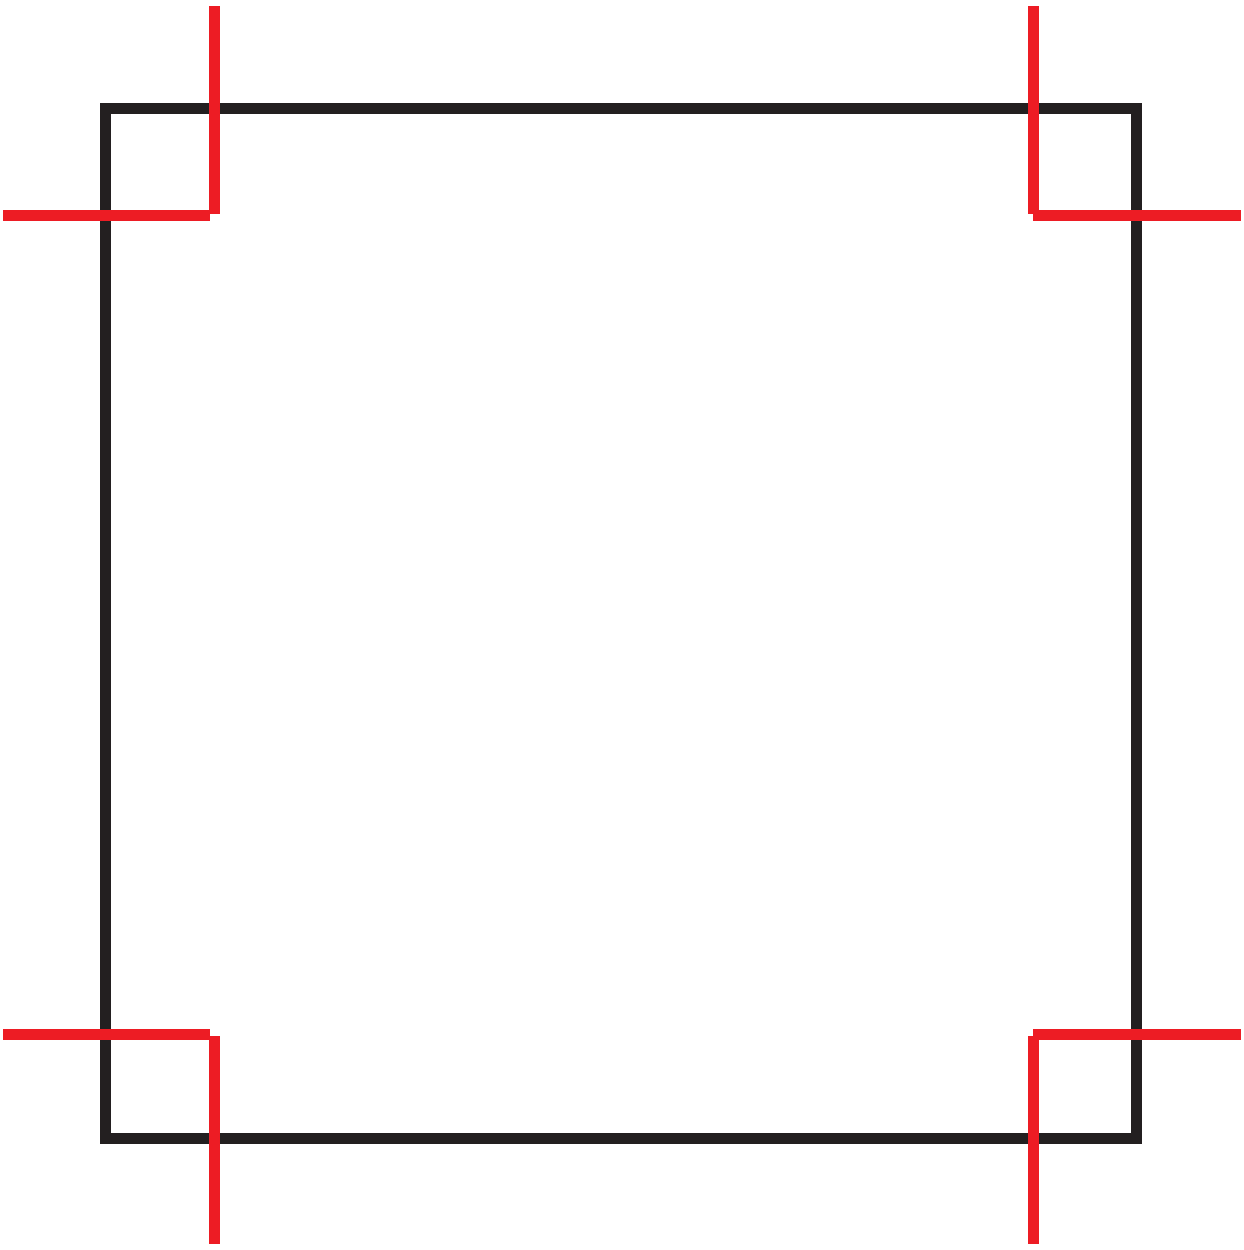
\includegraphics[width=0.3\textwidth]{Images/inflation_1.pdf}
\hspace{\fill}
\pause 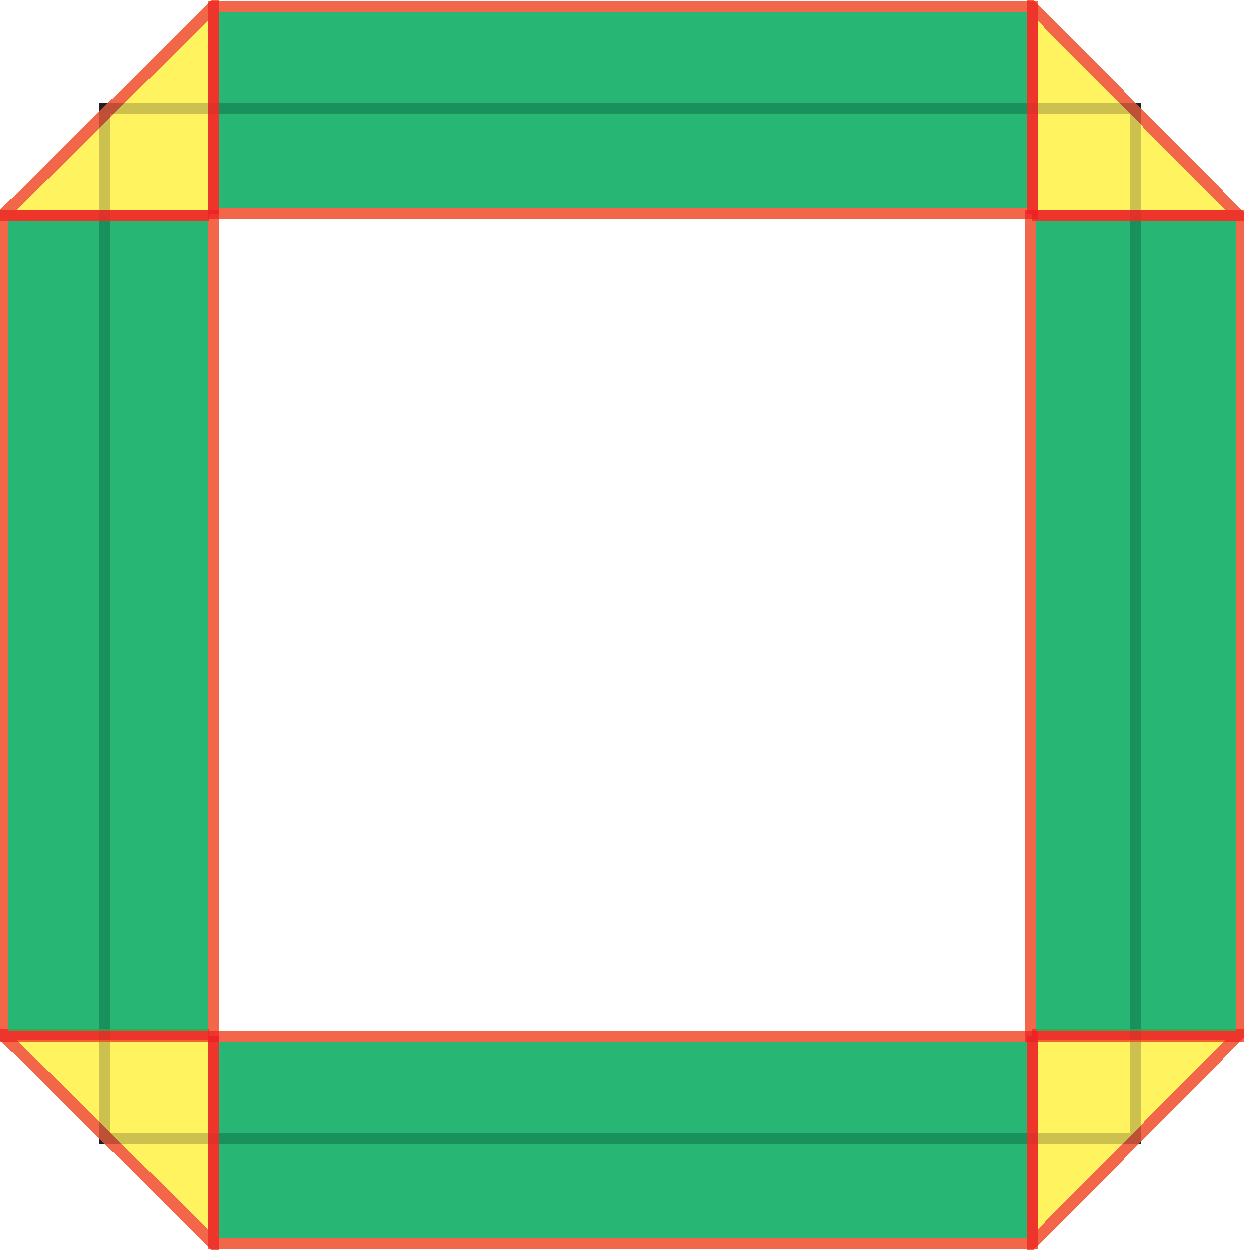
\includegraphics[width=0.3\textwidth]{Images/inflation_2.pdf}
\hspace{\fill}

\vspace{3mm}
\hspace{\fill}
\pause 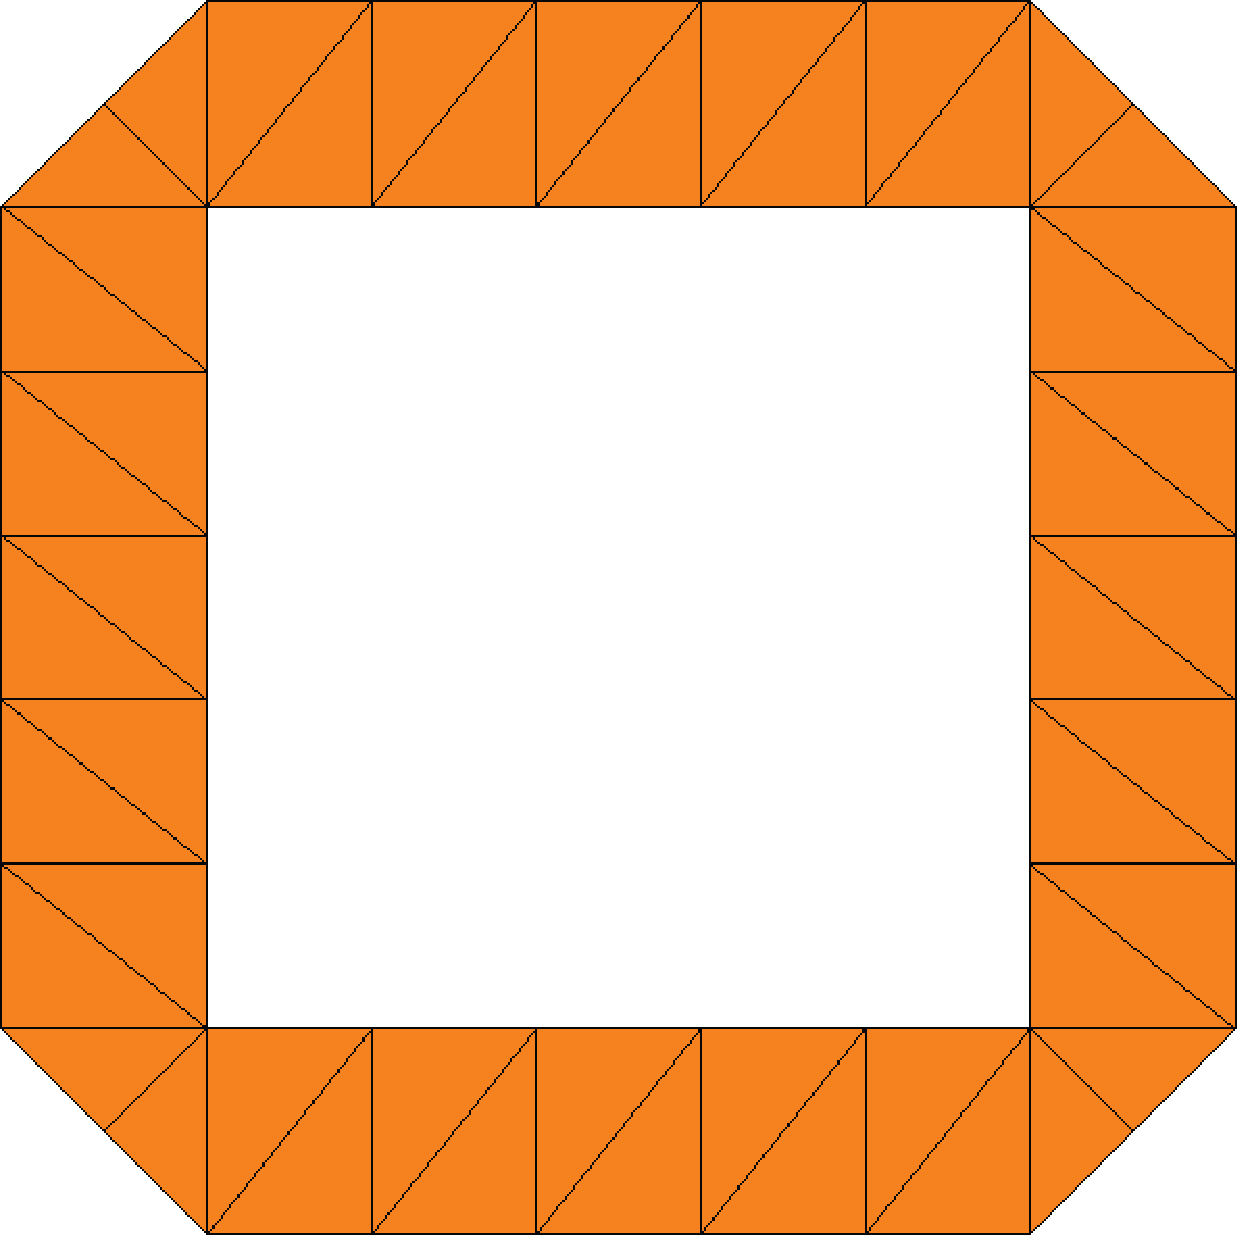
\includegraphics[width=0.3\textwidth]{Images/inflation_3.pdf}
\hspace{\fill}
\pause 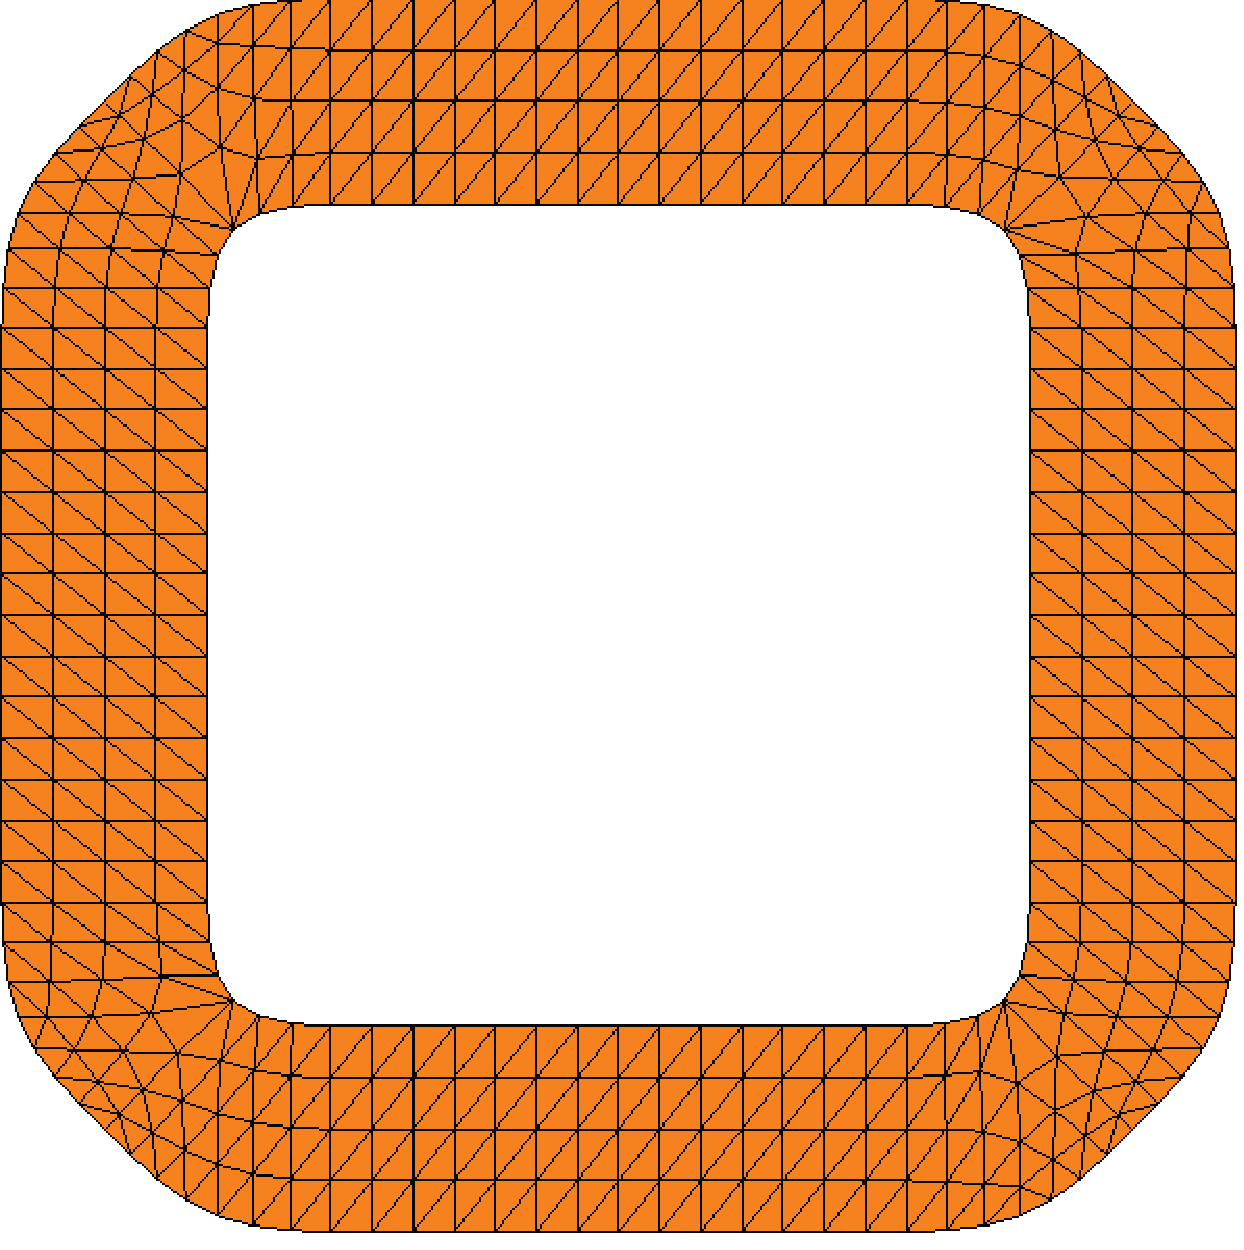
\includegraphics[width=0.3\textwidth]{Images/inflation_4.pdf}
\hspace{\fill}
\end{figure}
\end{frame}

\begin{frame}{Periodic inflation}
% Periodic inflation example
\begin{figure}
\hspace{\fill}
\includegraphics[width=0.4\textwidth]{Images/brick5_periodic.png}
\hspace{\fill}
\includegraphics[width=0.4\textwidth]{Images/star_periodic.png}
\hspace{\fill}

\vspace{3mm}
\hspace{\fill}
\includegraphics[width=0.4\textwidth]{Images/truncated_octahedron_periodic.png}
\hspace{\fill}
\includegraphics[width=0.4\textwidth]{Images/diamond_periodic.png}
\hspace{\fill}
\end{figure}
\end{frame}

\begin{frame}{Pattern parameters}
% Pattern parameters
\begin{figure}
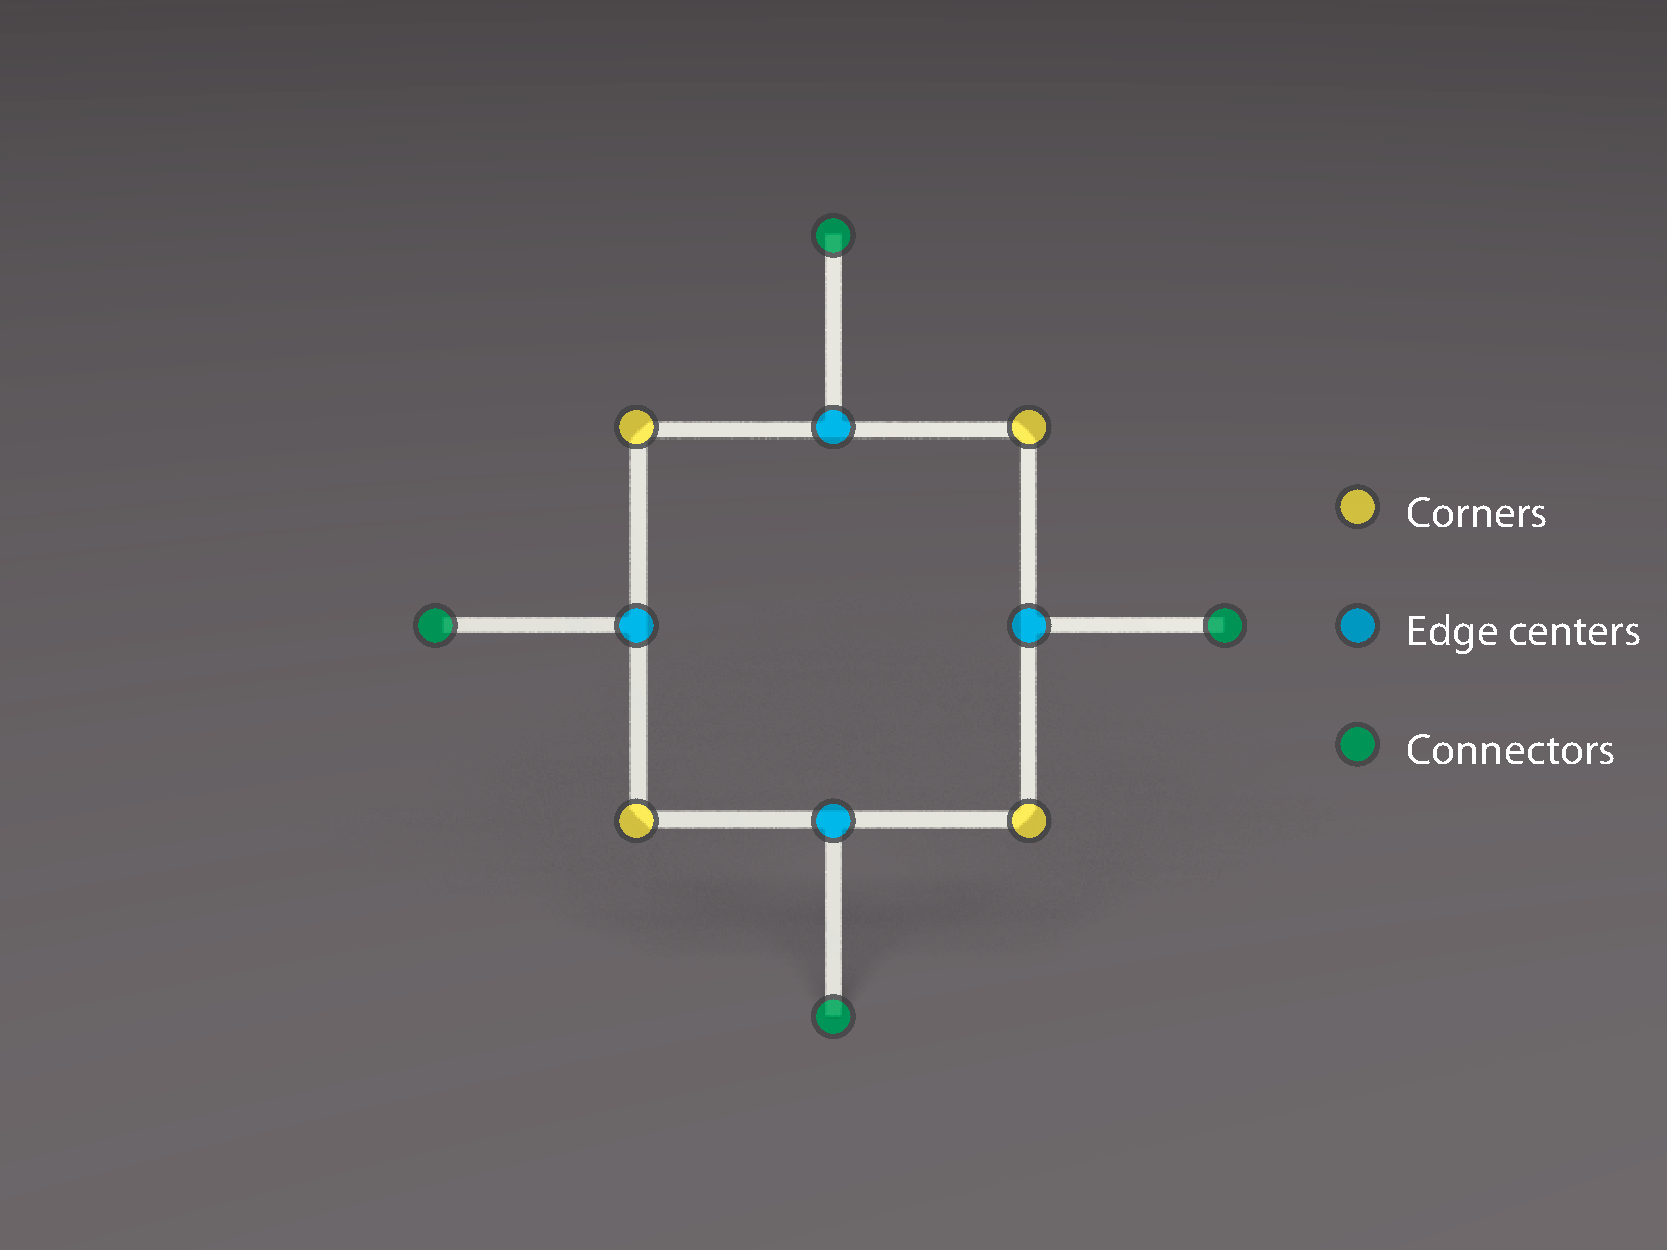
\includegraphics[width=0.9\textwidth]{Images/box_2D_parameters.pdf}
\end{figure}
\end{frame}

\begin{frame}{Pattern parameters}
\begin{figure}
\hspace{\fill}
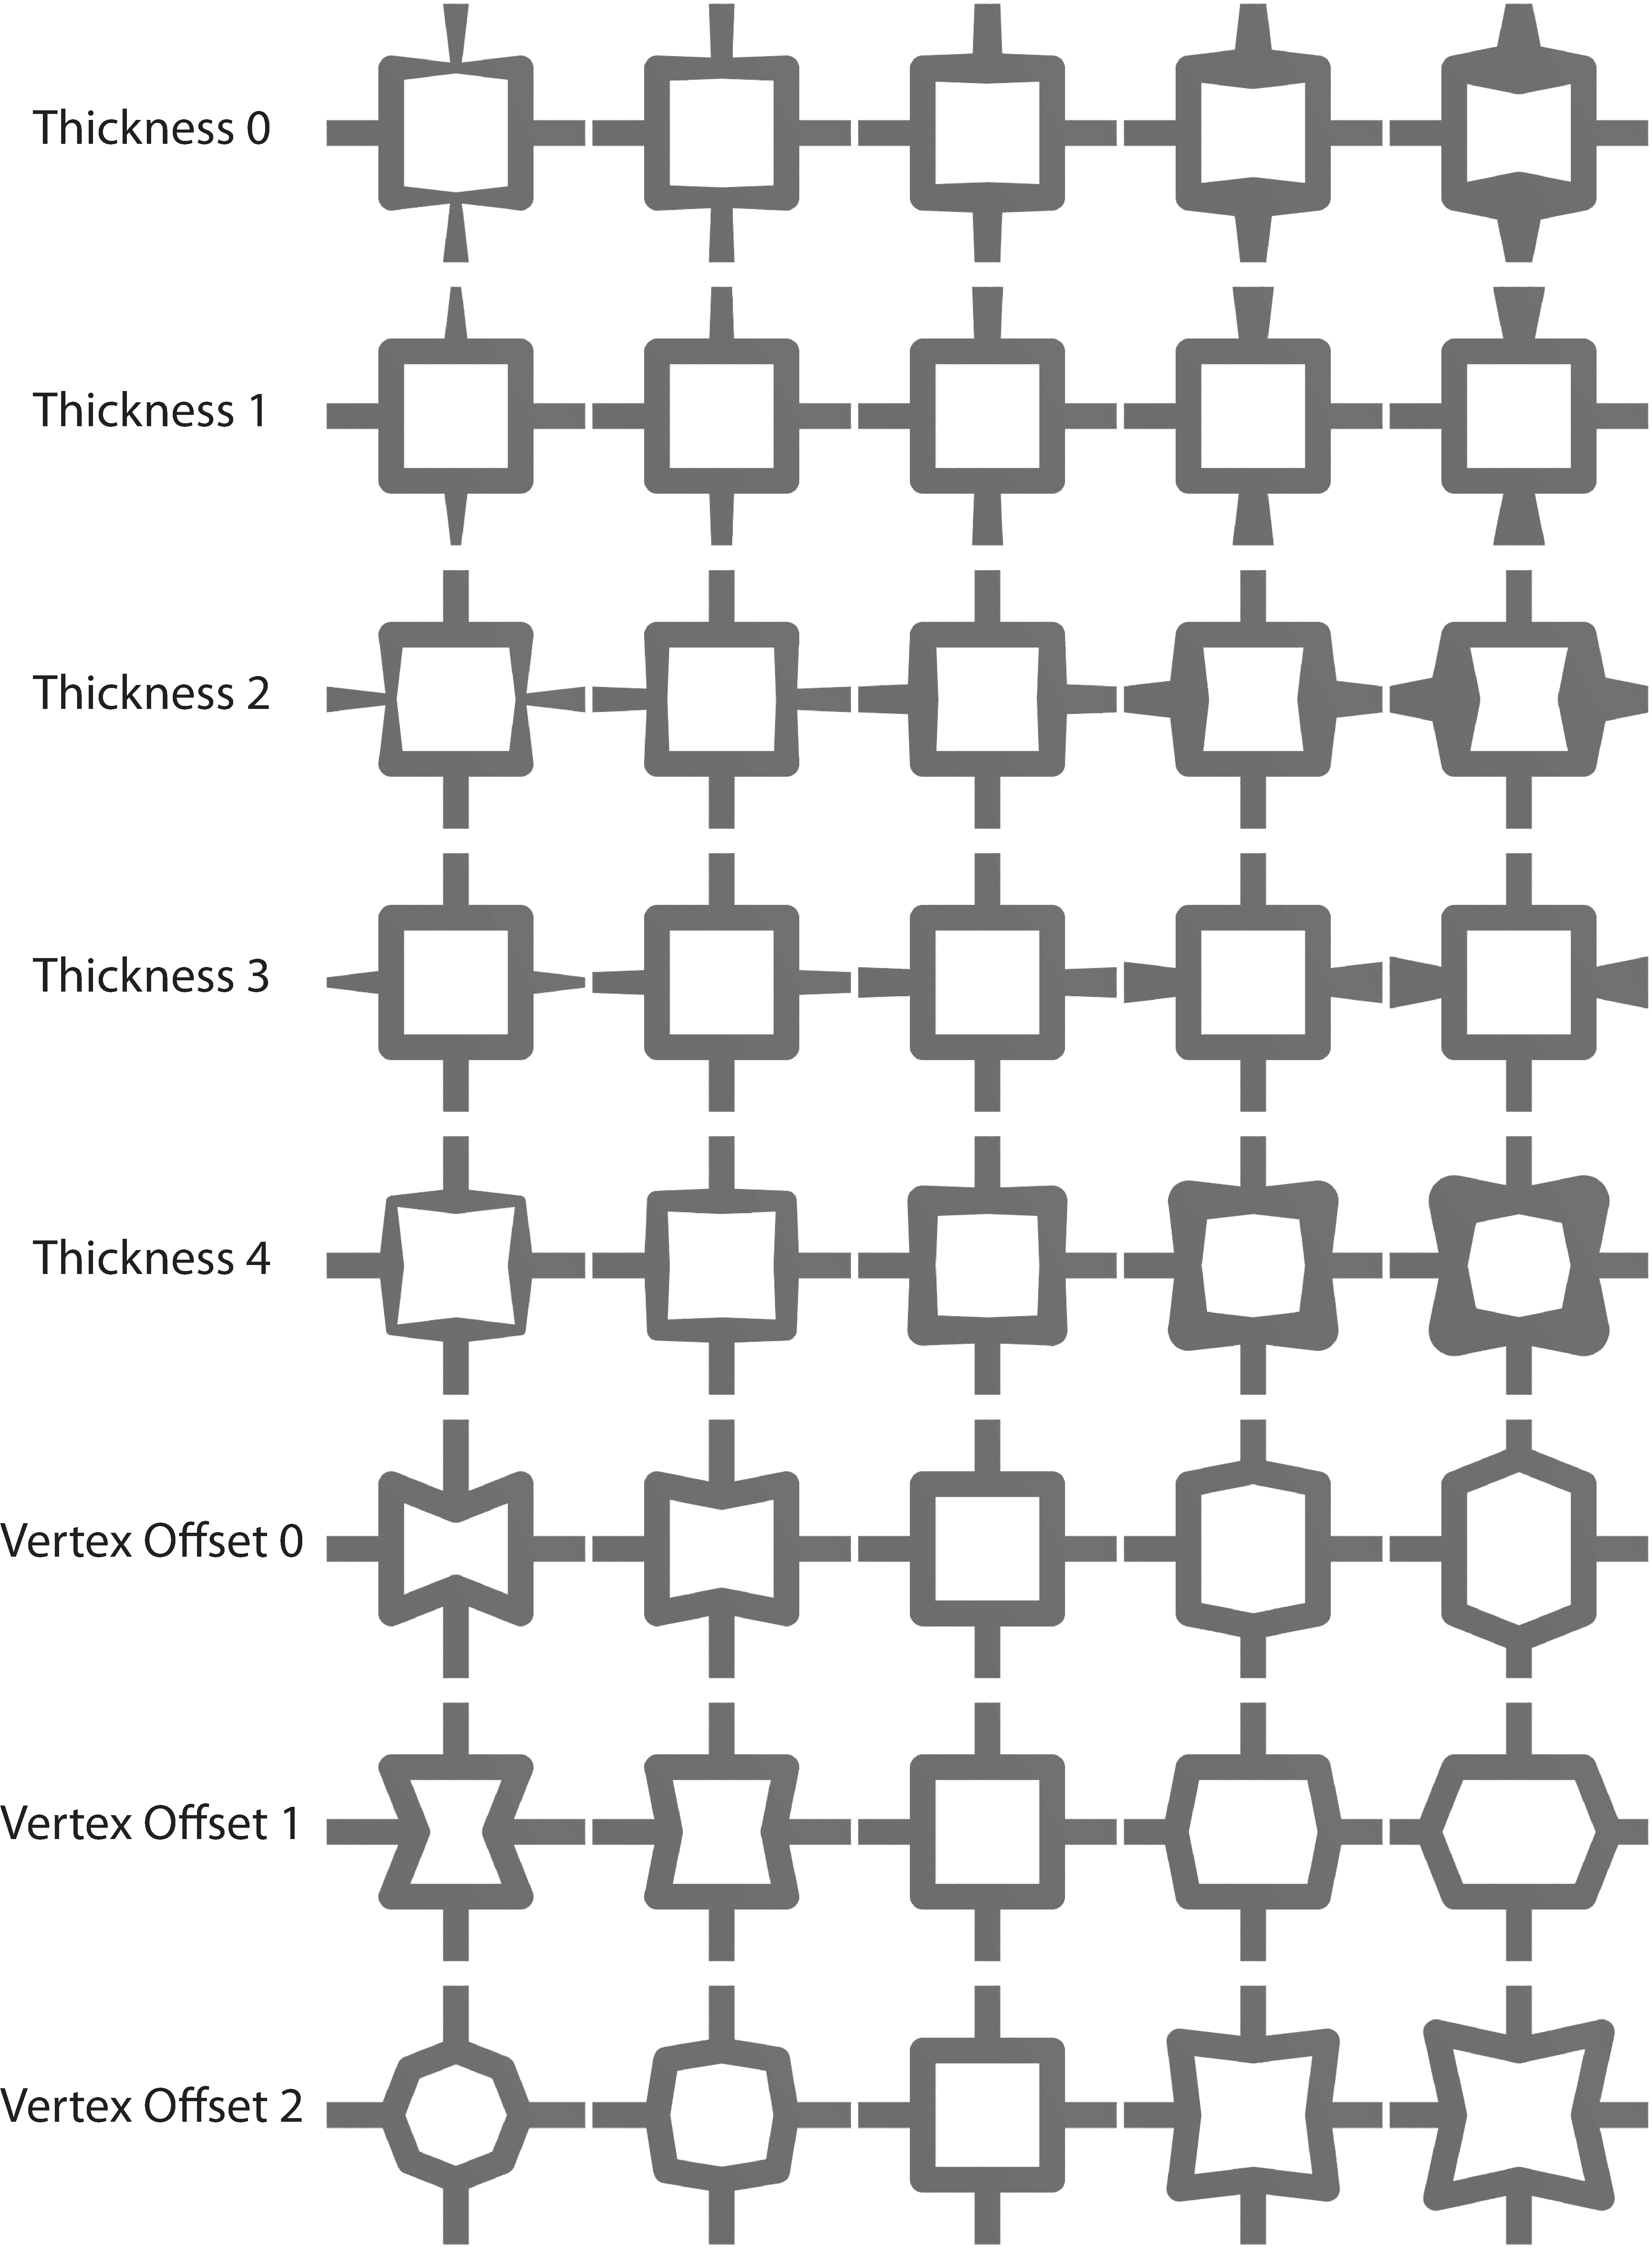
\includegraphics[height=0.8\textheight]{Images/box_2D_param.pdf}
\hspace{\fill}
\end{figure}
\end{frame}

%\begin{frame}{Pattern parameters}
%% Pattern parameters
%\begin{figure}
%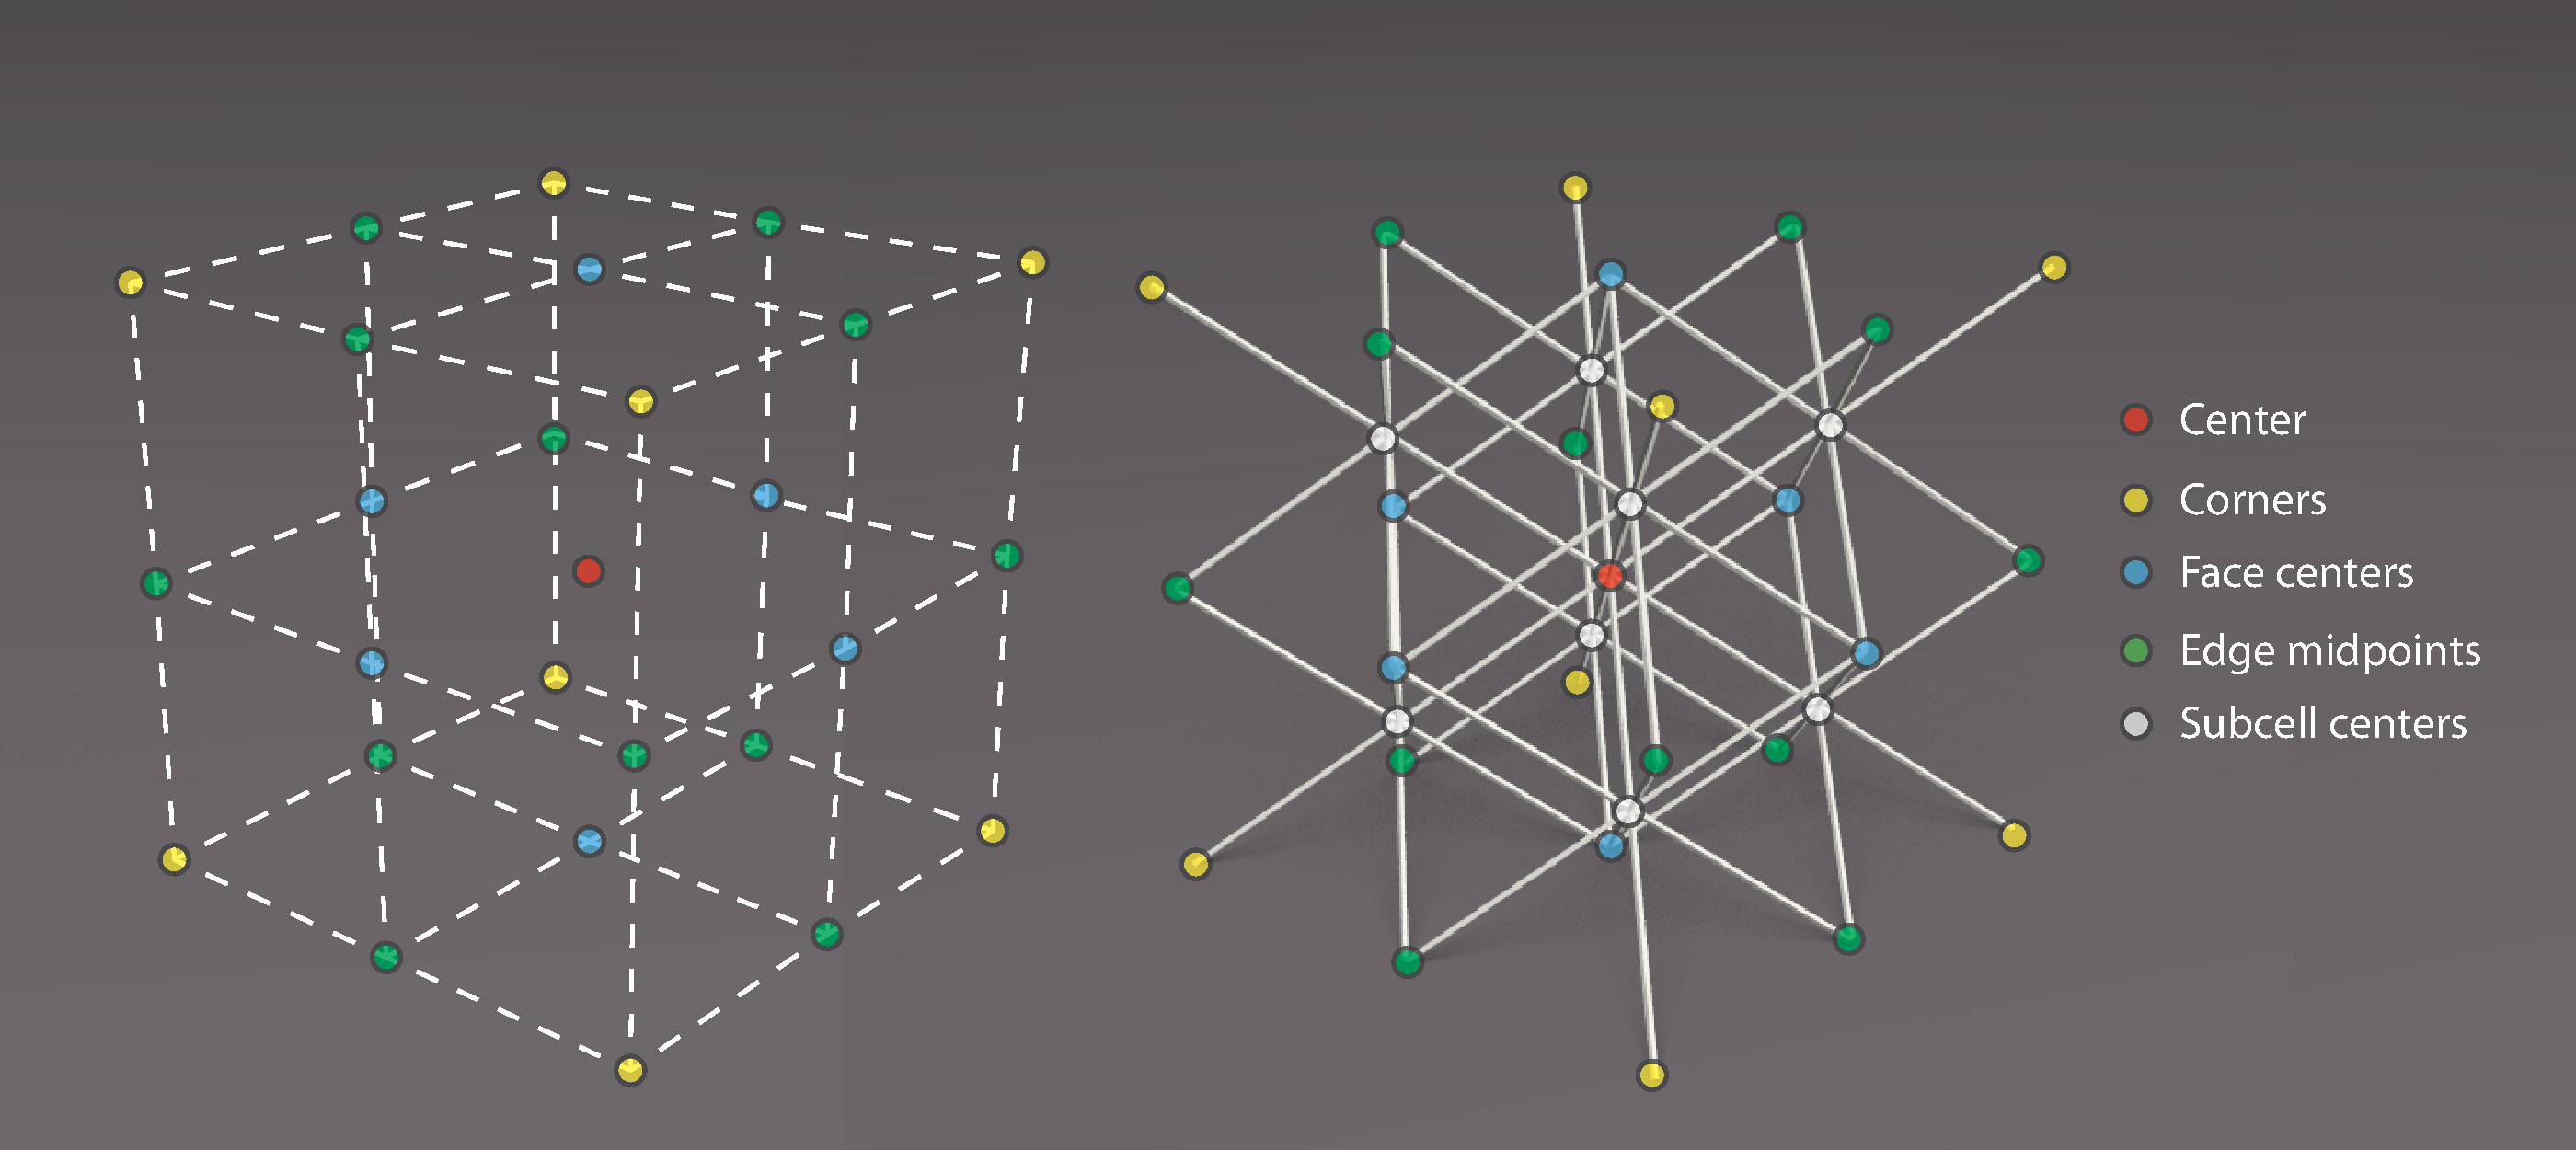
\includegraphics[width=0.9\textwidth]{Images/star_parameters.pdf}
%\end{figure}
%\end{frame}

\begin{frame}{Pattern parameters}
% Pattern parameters
\begin{figure}
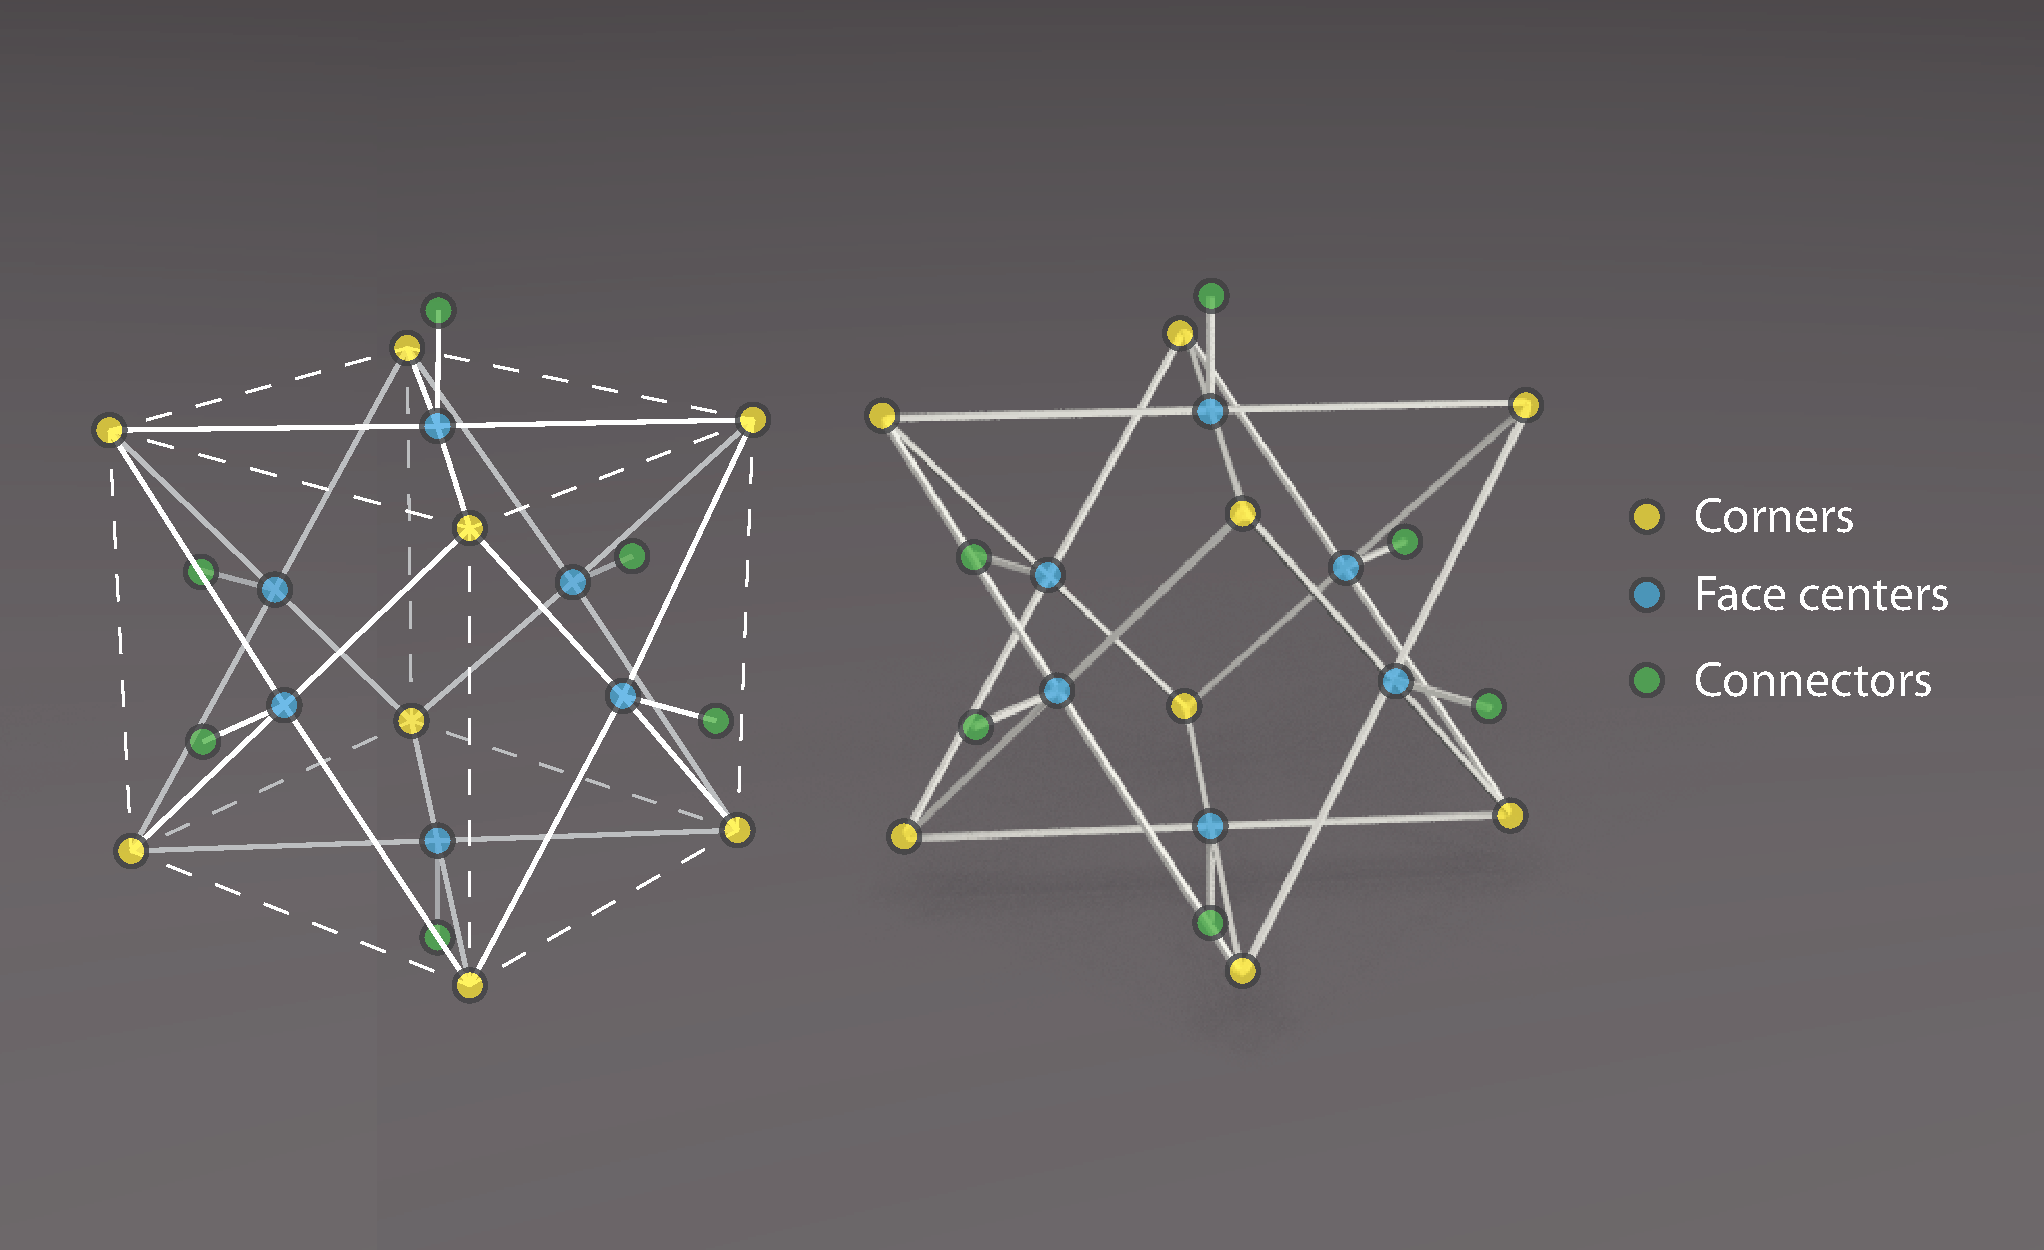
\includegraphics[width=0.9\textwidth]{Images/brick5_parameters.pdf}
\end{figure}
\end{frame}


\begin{frame}{Pattern parameters}
\begin{figure}
\hspace{\fill}
\includegraphics[width=0.9\textwidth]{Images/brick5_param.png}
\hspace{\fill}
\end{figure}
\end{frame}

\begin{frame}{Printibility}
Support structure is bad.
\begin{figure}
\includegraphics[width=0.95\textwidth]{Images/microstructure_support.png}
\end{figure}
\end{frame}

\begin{frame}{Printibility}
Pushing printers to its limit.
\begin{figure}
\includegraphics[height=0.8\textheight]{Images/microstructure_prints.pdf}
\end{figure}
\end{frame}

